\documentclass{beamer}
%Information to be included in the title page:
\title{Dynamic Programming}
\author[1705XXX, 1705XXX]{Peter Parker \\ 1705XXX \and \\ Tony Stark \\ 1705XXX}


\date{\today}
\usetheme{Berlin}
\usepackage{xcolor}
\usepackage{tikz}
\usetikzlibrary{positioning,shapes}



\begin{document}

\frame{\titlepage}

\begin{frame}{Tabe of Contents}
    \tableofcontents
\end{frame}

\section{Introduction}

\begin{frame}
\frametitle{We are going to see}

    \tableofcontents
\end{frame}
\begin{frame}{Dynamic Programming}
\begin{itemize}
    \item Algorithm technique that systematically records the answers
to sub-problems and reuses them those recorded result
\pause
\item A simple example: \\
Calculating the n-th Fibonacci number: \\
$Fib(n) = Fib(n-1) + Fib(n-2)$
\end{itemize}
\end{frame}
\setbeamercovered{transparent}
\begin{frame}{continued.}
\begin{itemize}
    \item The method was developed by Richard Bellman in the 1950s.
    \pause
    \item It breaks down a complicated problem into simpler
sub-problems in a recursive manner.
    \pause
    \item If optimal solutions can be found recursively for the
sub-problems, then it is said to have optimal substructure.
\end{itemize}
    
\end{frame}


\section{Properties}

\begin{frame}
\frametitle{We are going to see}

    \tableofcontents
\end{frame}

\begin{frame}{Properties of Dynamic Programming}
Such problem exhibits two properties:
\begin{itemize}
    \item \textbf{Optimal Substructure}
    \item \textbf{Overlapping sub-problems}
\end{itemize}
\end{frame}

\begin{frame}{Optimal Substructure}
    A problem is said to have optimal substructure if an optimal
solution can be constructed from optimal solutions of its
sub-problems.\\
e.g. in \color{blue} Floyd-Warshall \color{black} algorithm,  travelling from node i to j using
node k, dist[i][j]=dist[i][k]+dist[k][j]
\end{frame}

\begin{frame}{Overlapping sub-problems}
    A problem has overlapping sub-problems if finding its solution
involves solving the same sub-problem multiple times.\\
Example: Calculating n-th Fibonacci number $F (n)$
\end{frame}

\begin{frame}{Example of Overlapping sub-problems}
\begin{figure}
    \centering
    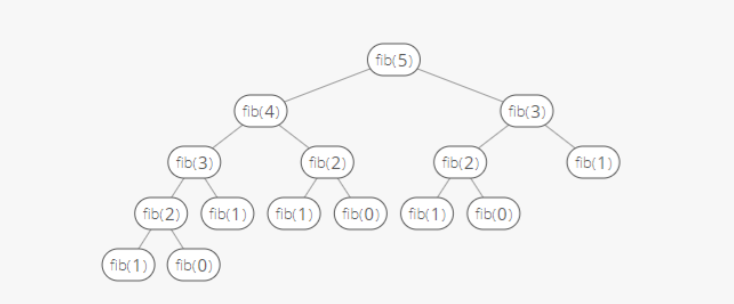
\includegraphics[scale = 0.5]{Fib.PNG}
    \caption{Overlapping Sub-problems in determination of Fibonacci series.}
    \label{fig:my_label}
\end{figure}

\end{frame}

\section{A Problem Solved Using DP}

\begin{frame}
\frametitle{We are going to see}

    \tableofcontents
\end{frame}

\begin{frame}{Binomial Coefficient a.k.a C(n,r)}
problem statement: \color{red} ways to select \color{black} r objects from n objects
regardless of the ordering 
\end{frame}

\begin{frame}
\frametitle{We are going to see}

    \tableofcontents
\end{frame}

\begin{frame}{Binomial Coefficient a.k.a C(n,r)}
\begin{columns}
\begin{column}{0.5\textwidth}
Naive approach: calculating \\
$\frac{n!}{r!(n-r)!}$
\end{column}
\begin{column}{0.5\textwidth}
\begin{itemize}
    \item Problem : overflow will be
caused calculating factorials,
unsigned long long wouldn’t
be enough. May be
BigInteger would do but not
efficient.
\item Solution : using dynamic
programming.
\end{itemize}
\end{column}
\end{columns}
\end{frame}

\begin{frame}{C(n,r) having dynamic programming properties}
    \textbf{Optimal Substructure:} C(n,r) can be recursively calculated using
the formula,\\
$C (n, r ) = C (n-1, r-1) + C (n-1, r )$\\
with base cases, $C(n,0) = C(n,n) = 1$ and $C(n,1) = n$ 
\end{frame}

\begin{frame}{C(n,r) having dynamic programming properties}
    \textbf{Overlapping Sub-problems: let n=5, r=2}
    \begin{center}
        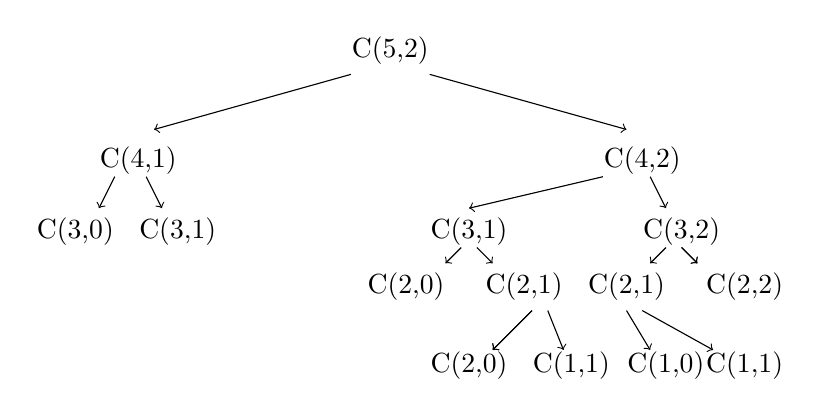
\begin{tikzpicture}
            \node at (0,0) {C(5,2)};
            \draw [->](-0.5,-0.3) -- (-3,-1);
            \draw [->](0.5,-0.3) -- (3,-1);
            \node at (-3.2,-1.4) {C(4,1)};
            \node at (3.2,-1.4) {C(4,2)};
            \draw [->](-3.5,-1.6) -- (-3.7,-2);
            \draw [->](-3.1,-1.6) -- (-2.9,-2);
            \draw [->](2.7,-1.6) -- (1,-2);
            \draw [->](3.3,-1.6) -- (3.5,-2);
            \draw [->](3.5,-2.5) -- (3.3,-2.7);
            \draw [->](3.7,-2.5) -- (3.9,-2.7);
            \draw [->](1.1,-2.5) -- (1.3,-2.7);
            \draw [->](0.9,-2.5) -- (0.7,-2.7);
            \draw [->](3.7,-2.5) -- (3.9,-2.7);
            \draw [->](2,-3.3) -- (2.2,-3.8);
            \draw [->](1.8,-3.3) -- (1.3,-3.8);
            \draw [->](1.8,-3.3) -- (1.3,-3.8);
            \draw [->](3,-3.3) -- (3.3,-3.8);
            \draw [->](3.2,-3.3) -- (4.1,-3.8);
            \node at (-4,-2.3) {C(3,0)};
            \node at (-2.7,-2.3) {C(3,1)};
            \node at (1,-2.3) {C(3,1)};
            \node at (3.7,-2.3) {C(3,2)};
            \node at (0.2,-3) {C(2,0)};
            \node at (1.7,-3) {C(2,1)};
            \node at (3.0,-3) {C(2,1)};
            \node at (4.5,-3) {C(2,2)};
            \node at (1,-4) {C(2,0)};
            \node at (2.3,-4) {C(1,1)};
            \node at (3.5,-4) {C(1,0)};
            \node at (4.5,-4) {C(1,1)};
        \end{tikzpicture}
    \end{center}
\end{frame}

\begin{frame}{}
    \begin{table}[]
\begin{tabular}{|llll|}
\hline
\multicolumn{4}{|c|}{Algorithm List}                                                                                       \\ \hline
\multicolumn{1}{|l|}{Algorithm Name} & \multicolumn{1}{l|}{} & \multicolumn{1}{l|}{Time Complexity}     & Space Complexity \\ \hline
\multicolumn{1}{|l|}{BFS}            & \multicolumn{1}{l|}{} & \multicolumn{1}{l|}{$O(|V|+|E|)$}        & $O(|V|)$         \\ \hline
\multicolumn{1}{|l|}{DFS}            & \multicolumn{1}{l|}{} & \multicolumn{1}{l|}{$O(|V|+|E|)$}        & $O(|V|)$         \\ \hline
\multicolumn{1}{|l|}{Dijkstra}       & \multicolumn{1}{l|}{} & \multicolumn{1}{l|}{$O(|V|+|E|\log|V|)$} & $(O|V|+|E|)$     \\ \hline
\multicolumn{1}{|l|}{Bellman Ford}   & \multicolumn{1}{l|}{} & \multicolumn{1}{l|}{$O(|V|*|E|)$}        & $O(|V|)$         \\ \hline
\multicolumn{1}{|l|}{Floyd-Warshall} & \multicolumn{1}{l|}{} & \multicolumn{1}{l|}{$O(|V|^3)$}          & $O(|V|^2)$       \\ \hline
\multicolumn{1}{|l|}{Edmonds-Karp}   & \multicolumn{1}{l|}{} & \multicolumn{1}{l|}{$O(|V|*|E|^2)$}      & $O(|V|+|E|)$     \\ \hline
\end{tabular}
\end{table}
\end{frame}

\end{document}